\documentclass[../index.tex]{subfiles}
\begin{document}
    Динамические формы позволяют объединять последовательности элементов в единые сущности, называемые группами. Группы можно объединять под единым заголовком, визуально "сворачивать/разворачивать", копировать и удалять.

\section{Виды групп}
        Существуют несколько видов групп: так называемые, <<legacy>> и <<плоские>> группы -- элементы логически объединенные общим идентификатором группировки -- формат SMIT и старых версий  ПО ДРУГа и многоуровневые или просто <<группы>> -- современный формат, поддерживаемый ПО ДРУГа и позволяющий описывать сложные древовидные структуры динамических форм. Среда выполнения dom-core
        приводит legacy-форматы групп к древовидным на время работы с обращением, при этом в некоторых случаях при сохранении может потребоваться обратное преобразование формата для поддержки совместимости со старыми системами.
\begin{enumerate}
    \item Плоские группы. Плоские группы представляют собой элементы, объединенные по параметру \textbf{groupid}. Такие группы не имеют заголовка, и визуально не отделяются от остальных элементов. Основная задача, которую решают данные группы -- сортировка и группировка элементов в одном блоке, поддерживающим операции копирования и удаления. При работе через dom-core всегда требуется обратное преобразование в исходный формат.
    \item Legacy группы. Основное отличие от плоских групп заключается в наличии заголовка. Есть отличительная особенность поддержки Legacy групп Лице Друга 1.0 и domcore: в первом случае поддерживается наличие более одного заголовка в группе, во втором же принято решение, что заголовок группы может быть один. Все остальные заголовки не обрезаются при обработке динамической формы. При визуализации Legacy Group могут сворачиваться и управляться командой динамического языка \textbf{setFocus}. При сохранении через dom-core они могут не разворачиваться и отправляться как нормальные группы, за исключением шаблонов помеченных атрибутом needunwrap, требующего развернуть
    \item Группы. Целевой механизм групп. В xml-представлении ПО ДРУГа представлен элементом \verb|<group>|, поддерживащим вложенные
    динамические элементы. Количество и тип вложенных элементов не ограничены: это могут быть и другие группы, что позволяет создавать сложные иерархические структуры динамических элементов. В json-представлении описываются массивом с именем \verb|"childs"|.
\end{enumerate}

\section{Копирование групп}
Копирование групп -- стандартная функциональность, поддерживаемый динамическим языком и позволяющий <<тиражировать>> элементы динамической формы, объединенные в группу. Копирование группы вызывается командой динамического языка \textbf{copyGroup} (\autoref{copygroupgroupid-id-group-string}, \autopageref{copygroupgroupid-id-group-string}). Принято прописывать копирование группы либо в <<sbcommand>>, либо в <<sbtask>> атрибуте кнопки <<addButton>>.
Функциональность копирования групп привязана к исходному (шаблонному) состоянию элементов в динамической форме, а не к их состоянию в момент копирования.
Рассмотрим механизм копирования групп на примере представленного ниже json-представления шаблона:
\begin{verbatim}
{
    "objectType": "group",
    "logicalType": "group",
    "id": "groupaddress",
    "label": "Пункт отправления/прибытия",
    "mandatory": false,
    "style": "group",
    "visible": true,
    "width": "",
    "sbdbfield": "groupAddressTo",
    "sbonload": "",
    "sbcopyinfo": false,
    "childs": [
        {
        "objectType": "select",
        "logicalType": "combo",
        "id": "addressto",
        "label": "Маршрут следования",
        "mandatory": true,
        "sbcommand": "",
        "sbmask": "",
        "sbmodify": true,
        "sbtask": "if(
    [run(
        [setValue(
            [getDistance(
                [getValues([find([id],[address],[grouptrip])]
                )]
            )],
            [array]
        )]
    )],
[if(
    [isin(
        [getText(  [distance], [array] )], []
    )],
    [run( [clear( [array])],
        [setValue( [0,00], [cost])],
        [setValue(
            [plus(
                [#0.00],
                [getTexts([find([id],[plus([c],[ost])],[])])]
            )],
            [allcost]
        )],
        [setValue([0,000], [distancetext]
        )],
        [setValue( [0], [timetext])],
        [setValue([0], [distancevalue])],
        [setValue( [0], [kmdistancevalue] )],
        [setValue( [0], [timevalue])],
        [setValue(
        [plus(
            [#0.000],
            [div( [#0.000],[plus( [#0.000],
            [getTexts(
                    [find([id],
                         [plus([distanc],[evalue])],[])])]
                    )],
                [1000]
            )]
        )],
        [alldistancetext]
        )],
        [setValue(
            [plus(
                [div( [#0], [plus( [#0.00],[getTexts(
                 [find([id],
                     [plus([tim],[evalue])],[])])])],[60]
                )]
            )],
            [alltimetext]
        )]
    )],
[run(
    [setValue(
        [getText([time_text], [array])],
        [timetext]
    )],
    [setValue(
        [div(
            [#0.000],
            [getText([distance], [array])],
            [1000]
        )],
        [distancetext]
    )],
    [setValue(
        [getText([time], [array])],
        [timevalue]
    )],
    [setValue(
        [getText([distance],[array] )],
        [distancevalue]
    )],
    [setValue(
        [div(
            [#0.000],
            [getText([distance], [array])],
            [1000]
        )],
        [kmdistancevalue]
    )],
[if(
    [run(
        [setValid([true],[], [pricelabel])],
        [setValues(
            [_getCost(
                [FF_GET_CONDITIONAL_PRICE_DOUBLE],
                [getUser( [TabNum])],
                [getText([distance], [array])],
                [getText([time], [array])],
                [getText([cfgtransporttype] )],
                [plus([#0.00],
                  [getTexts([find([id],[wait],[grouptrip])])])],
                [cost],[1],
                [getValue( [date])],
                [getUser([template])]
            )],
            [cost]
    )]
)],
[run(
    [setValue(
        [plus([#0.00],
            [getTexts([find([id],[plus([c],[ost])],[])])]
        )],
        [allcost]
    )],
    [setValue(
        [plus( [#0.000],[div([#0.000], [plus( [#0.000],
        [getTexts([find([id],
            [plus([distanc],[evalue])],[])])])],[1000])]
        )],
        [alldistancetext]
    )],
    [setValue(
        [plus([div([#0], [plus([#0.00], [getTexts(
            [find([id], [plus([tim],[evalue])],[])])])],[60])]
        )],
        [alltimetext]
    )]
)], [])])])],[])",
        "sbtitle": "",
        "sbtype": "address",
        "style": "combo",
        "groupid": ""
        },
        {
        "objectType": "text",
        "logicalType": "date",
        "id": "wait",
        "label": "Время ожидания",
        "mandatory": false,
        "sbcommand": "run(
    [setMinHours(
        [0],
        [setMaxHours([2],[this])]
    )],
    [if(
        [isin(
            [getValue([cfgtransporttype] )],
            [Такси]
        )],
        [setVisible([true],[this])],
        [setVisible([false],[this])]
    )]
)",
        "sbmask": "HH:mm",
        "sbmodify": true,
        "sbtask": "",
        "style": "text",
        "visible": false,
        "sbcopyinfo": false,
        "groupid": "distanation"
        },
        {
        "objectType": "checkbox",
        "logicalType": "buttonAdd",
        "id": "addgroupaddress",
        "label": "Добавить еще один адрес",
        "mandatory": false,
        "sbmodify": true,
        "sbtask": "copyGroup([groupaddress],[this])",
        "sbtype": "buttonadd",
        "style": "checkbox",
        "visible": true,
        "sbdbfield": "addGroupAddress",
        "text": "",
        "groupid": "distanation"
        }
    ]
}
\end{verbatim}

Пользователь заполняет значения <<Маршрут следования>> и <<Время ожидания>>, и при нажатии на кнопку <<Добавить еще один адрес» выполняется команда <<sbtask>>, в которой вызывается копирование группы. При этом, все заполненные ранее поля не учитываются: значения полей в скопированных элементах <<Маршрут следования>> и <<Время ожидания>> группе будут пустыми. Также не будут копироваться никакие динамические элементы, добавленные динамически. При копировании не учитываются никакие изменения, произведенные с элементами группы и самой группой. В том числе не учитываются изменения видимости, обязательности, возможности изменений и т.д.

\begin{figure}[h]
    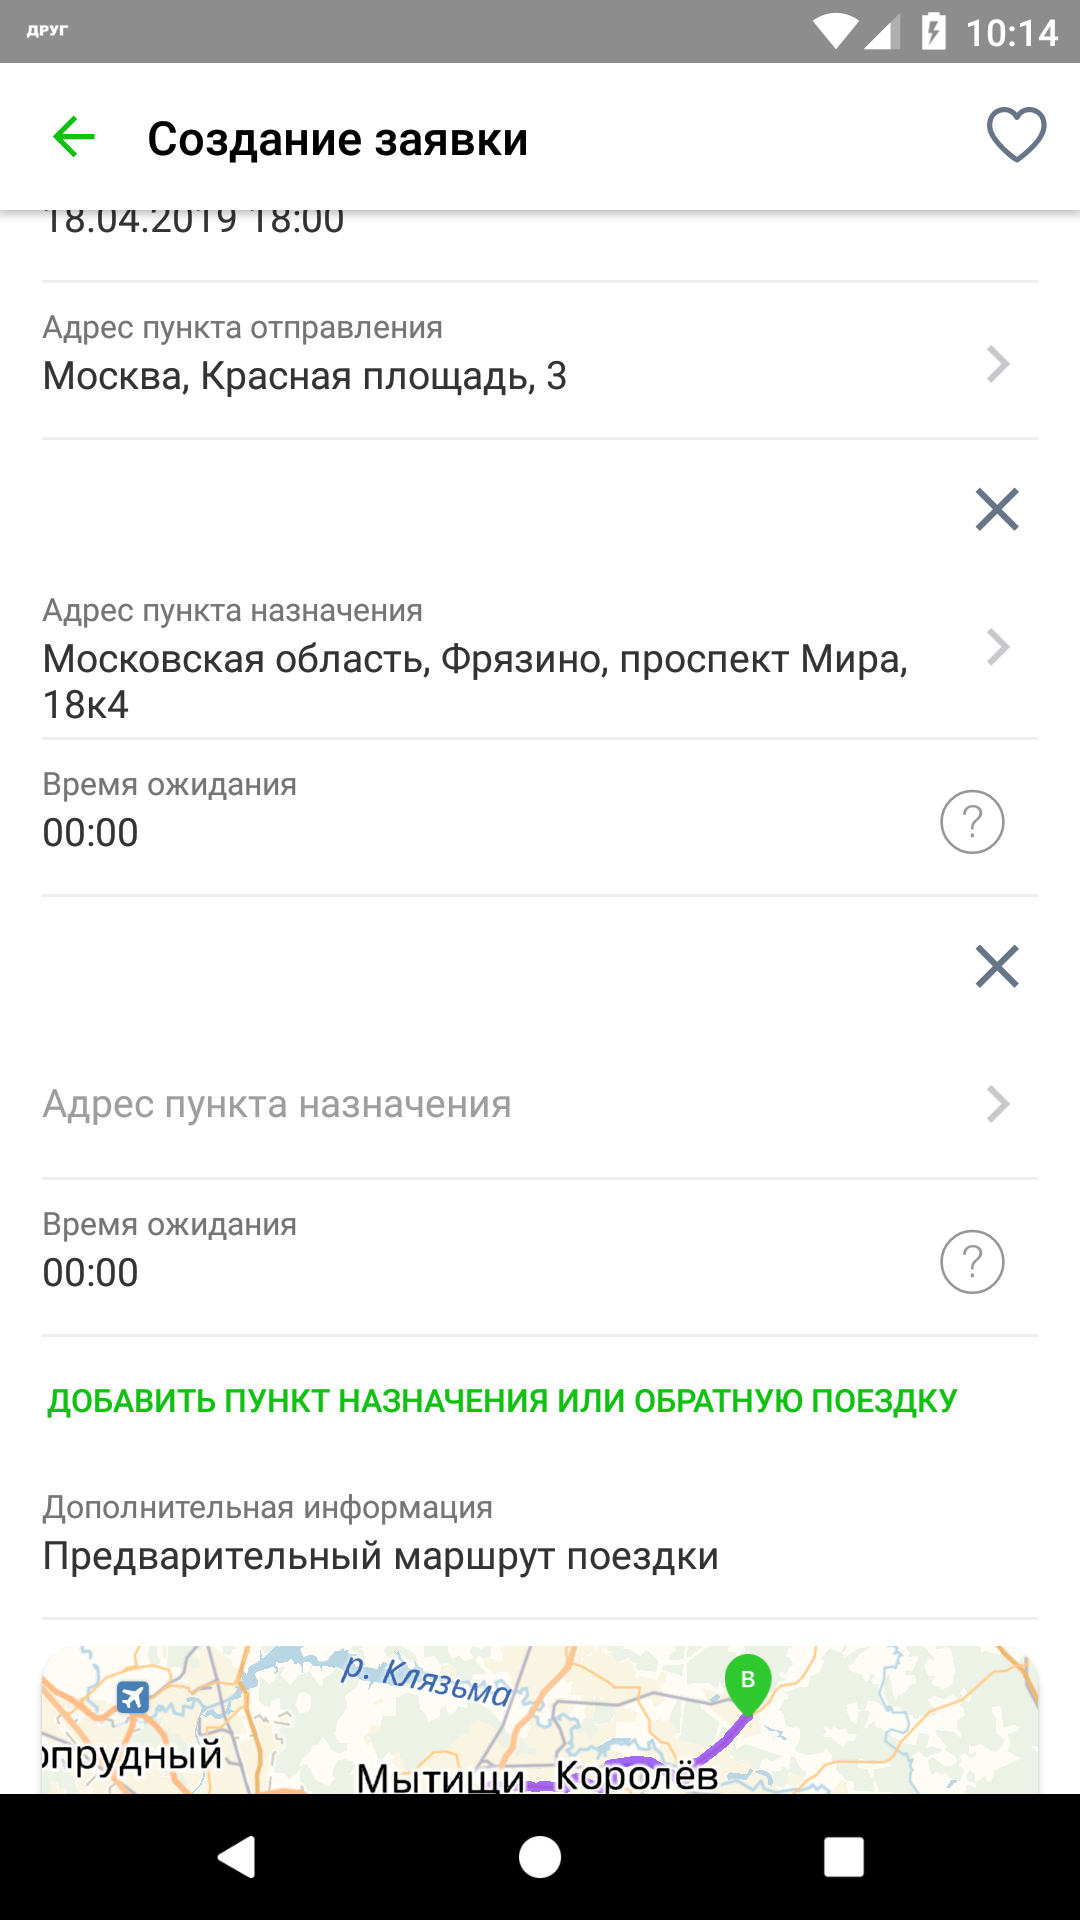
\includegraphics[width=0.4\textwidth]{copy_flat_group_mobile}
    \centering
    \caption{Пример копирования плоской группы в мобильном клиенте}
\end{figure}

\begin{figure}[h]
    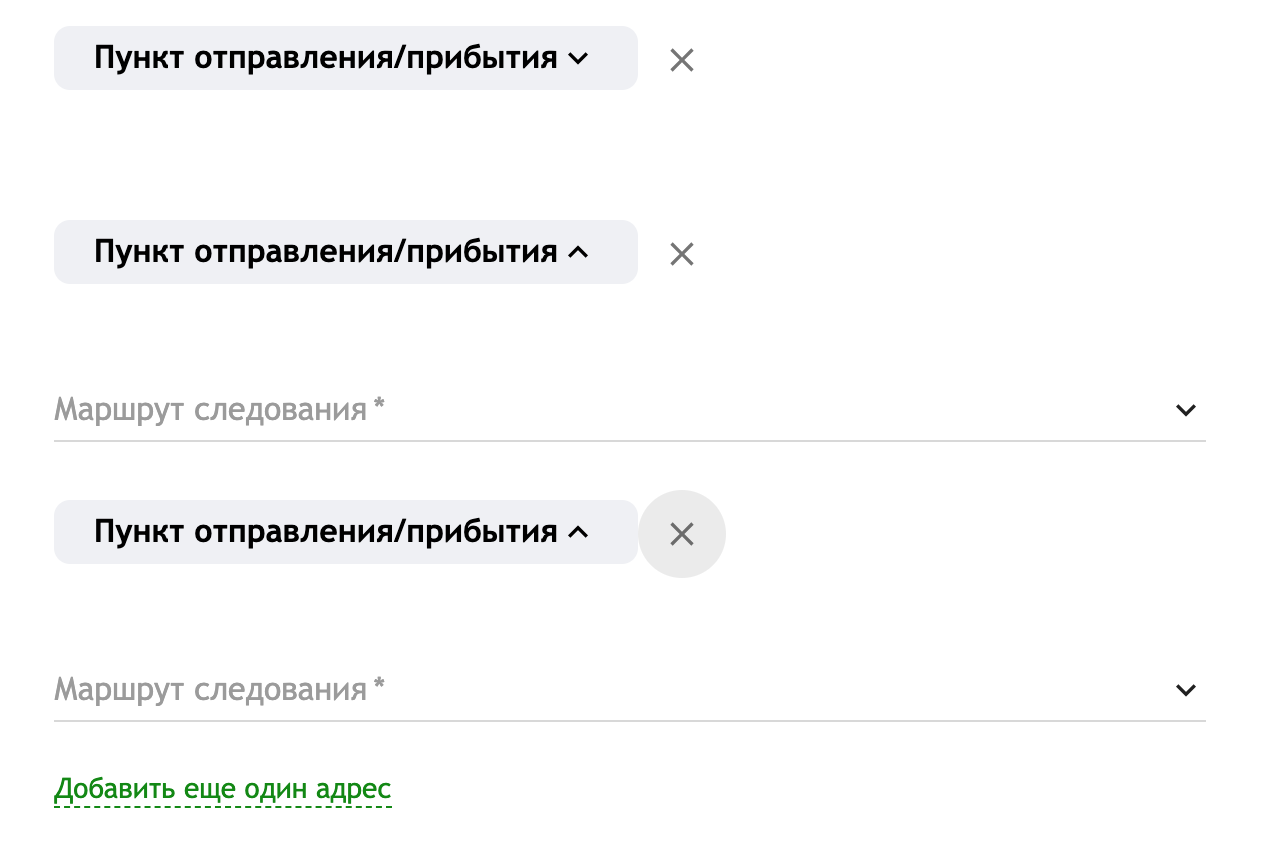
\includegraphics[width=0.4\textwidth]{copy_simple_group_face20}
    \centering
    \caption{Пример копирования и заголовков группы в интерфейсе Лицо 2.0}
\end{figure}

Еще одной важной особенностью является визуальное отображения кнопок копирования. Визуально все кнопки для копирования групп скрываются, кроме последней в наборе.
Исключительной особенностью обладают группы, элементы которых помещаются в одну строчку. Визуальное отображение элементов отделено от функционального. Если элементы группы для всех скопированных групп из одного множества удовлетворяют условию, что все элементы по ширине могу уместиться в одной строке(кнопка для копирования группы не учитывается при вычислениях), то визуально все группы склеиваются в одну и отображаются как общая группа с одним заголовком, при этом функциональная часть остается неизменной, там все также это представляется как разные группы.
Если копирование работает над <<Плоской>> группой -- проверять условия описанные выше не имеет смысла, так как плоские группы не имеют заголовка, поэтому проверка производится только для групп типа <<Legacy>> и стандартных групп.

\section{Удаление групп}

Удаление групп возможно только в том случае, если групп в подмножестве больше, чем одна. При добавлении группы через копирование у всех групп появляется возможность удалить группу через пользовательский интерфейс. Функция удаления -- одна из немногих, которые не поддерживается на уровне команд динамического языка, а разрешаются с использованием вызовов обработчиков через UI.

При нажатии на кнопку закрытия (крестик), происходит удаление группы. Если удаляемая группа содержит элемент \textbf{buttonAdd}, то после выполнения закрытия, выполняется динамическая команда, установленная в параметр \textbf{text} этого поля. В рассмотренном ранее примере, данный механизм позволяет пересчитать расстояния и стоимость поездки при удалении адреса из маршрута.

\end{document}
